\documentclass[slovene,11pt,a4paper]{article}
\usepackage[margin=1.8cm,bottom=3cm,foot=1.5cm]{geometry}
\usepackage{amsmath}
\usepackage{booktabs}
\usepackage{float}
\usepackage{graphicx}
\usepackage{gensymb}
\usepackage{geometry}
\usepackage{changepage}
\usepackage{subcaption}
\usepackage{multirow}
\usepackage{blindtext}
\usepackage{hyperref}
\usepackage[version=4]{mhchem}
\usepackage[slovene]{babel}
\pagenumbering{gobble}
\renewcommand{\contentsname}{\centering Contents}

\begin{document}

\title{5. naloga - Modeli kemijskih reakcij}
\author{Tadej Lozej 28201055}
\maketitle
\begin{center}
Modelska analiza 1 \\
\bigskip
Predavatelj: prof. dr. Simon Širca \\
Asistent: doc. dr. Miha Mihovilovič
\end{center}

\newpage

\tableofcontents

\newpage

\section{Uvod}

\pagenumbering{arabic}

V nalogi se ukvarjamo s modeliranjem kemijskih reakcij. Ogledamo si tri različne reakcije in spremljamo koncentracije različnih reaktantov in produktov v odvisnosti od časa. Kemijske reakcije obranvamo na način iz katerega smo izključili vso naključnost. Preprosto zapišemo sistem diferencialnih enačb in ga rešimo. Sisteme diferencialnih enačb nato rešujemo lahko eksaktno ali v priblićku stacionarnega stanja.

\section{Binarna reakcija}

Obravnavamo model binarne kemijske reakcije

\begin{align}
\ce{A + A <=>[p][q] A + A^*} \\
\ce{A^* ->[r] B + C}.
\end{align}
V shemi reakcije parametri $p$, $q$ in $r$ določajo hitrost s katero določena reakcija poteče. Sistem diferencialnih enačb, ki opisuje to kemijski reakcijo oz. sistem kemijskih reakcij je

\begin{align}
\dot{[A]} &= -p [A]^2 + q[A][A^*] \\
\dot{[A^*]} &= p [A]^2 - q [A][A^*] - r[A^*] \\
\dot{[B]} &= \dot{[C]} = r [A^*],
\end{align}
kjer so z oglatimi oglepaji označene koncentracije določene spojine ali elementa. Z uvedbo brezdimenzijskih spremenljivk

\[
a(t) = \frac{[A](t)}{[A](0)}, \quad a^*(t) = \frac{[A]^*(t)}{[A](0)}, \quad 
b(t) = \frac{[B](t)}{[A](0)}, \quad c(t) = \frac{[C](t)}{[A](0)}, \quad k = \frac{q}{p} \quad
\text{in} \quad s = \frac{r}{q[A](0)}
\]
lahko sistem diferencialnih enačb (3)-(5) lahko prepišemo v brezdimenzijski

\begin{align}
\dot{a} &= -a^2 + kaa^* \\
\dot{a^*} &= a^2 - kaa^* - ksa^* \\
\dot{b} &= \dot{c} = ksa^*,
\end{align}
kjer je s piko $\dot{}$ sedaj označen odvod po novem brezdimenzijskem času $t = p[A](0)t'$. Za vrednosti parametrov sledimo navodilom naloge. Vzamemo $k = 1000$ in $s = 10, 1, 0.1$. Sistem diferencialnih enačb (6)-(8) z omenjenimi vrednostmi parametrov rešimo v \texttt{Python}-u s funkcijo \texttt{scipy.integrate.solve\_ivp}, ki nam numerično reši problem takšnega tipa. Za numerični integrator izberemo \texttt{DOP853}, ki je metoda osmega reda. Na sliki 1 so prikazane rešitve sistema diferencialnih enačb (6)-(8). Vidimo, da manjši kot je  parameter $s$ počasneje pridemo do končnega stanja. To lahko razložimo, saj če je $s$ manjši je manjša hitrost reakcije (2) in večja hitrost v levo reakcije (1). Prav tako vidimo, da je vmesnega produkta $a^*$ za izbrane parametre ob vseh časih zelo malo. Ne samo, da ga je malo, ampak tudi zelo počasi spreminja svojo vrednost. Sploh pri večjih $s$ koncentracija vmesnega produkta $a^*$ konstantno zelo manjha. Ob tej opazki začnemo razmišljati o stacionarnem približku in njegovi upravičenosti.

\newpage

\begin{figure}[h!]
\centering
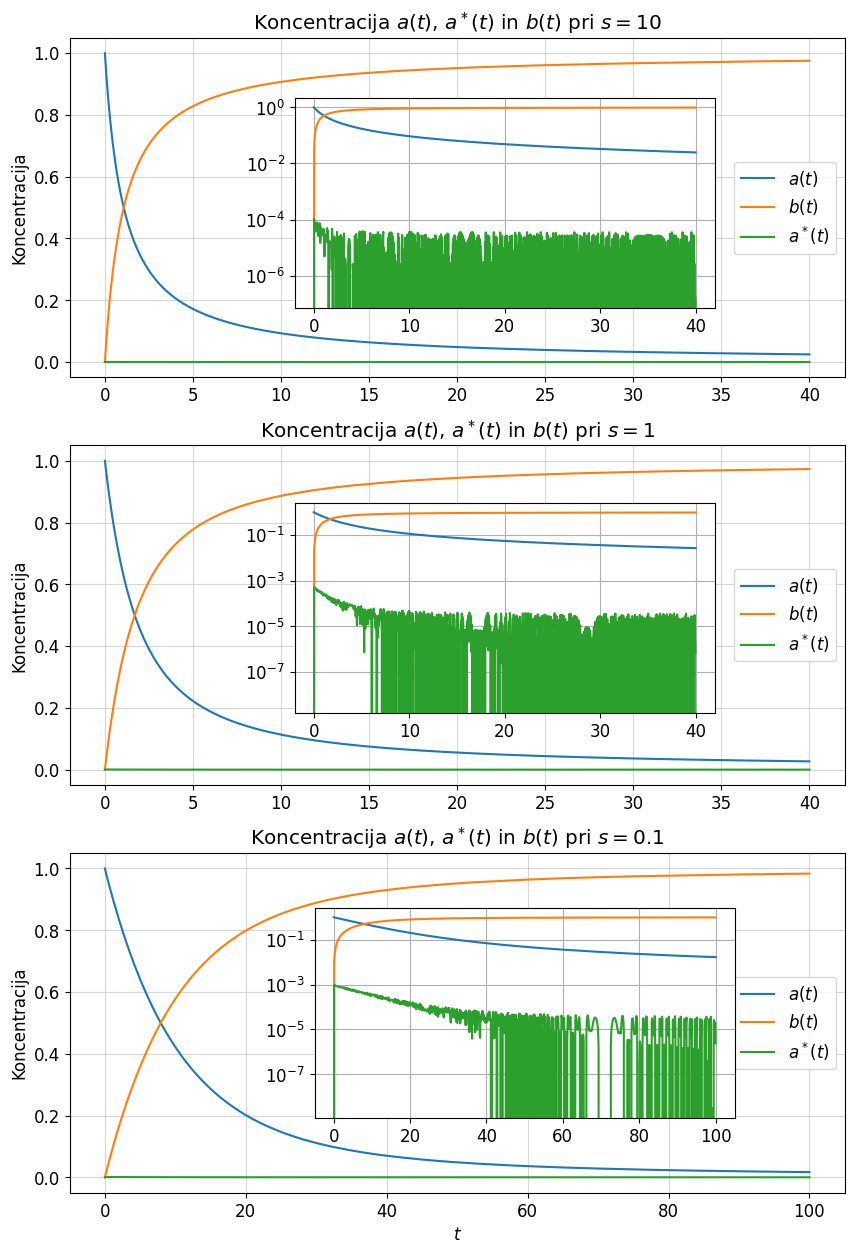
\includegraphics[width=15cm]{binarna1.png}
\caption{Na sliki vidimo potek koncentracij $a$, $b$ in $a^*$ v odvisnosti od časa pri različnih vrednostih parametra $s$. Vrednosti so prikazane v linearni in logaritemski skali. Vidimo, da za manjše $s$ reakcija poteka več časa. Prav tako je pomembna opazka ta, da se koncentracija vmesnega produkta $a^*$ zelo malo in počasi spreminja.}
\end{figure}

\newpage

\subsection{Stacionarni približek}

Ob opazovanju poteka koncentracij v odvisnosti od časa nam pade na pamet uporaba stacionarnega približka na vmesnem produktu $a^*$, saj se ta zelo malo in počasi spreminja. To pomeni, da v sistemu diferencialnih enačb (3)-(5) postavimo $\dot{[A^*]} = 0$, iz te enačbe izrazimo

\begin{equation}
[A^*] = \frac{p[A]^2}{q[A]+r}
\end{equation}
in ga vstavimo v drugi dve enačbi. Dobimo sistem dveh diferencialnih enačb, ki ga z brezdimenzijskimi spremenljivkami zapišemo kot

\begin{align}
\dot{a} = -\frac{sa^2}{a+s} \\
\dot{b} = \frac{sa^2}{a+s}.
\end{align}

Namesto sistema treh diferencialnih enačb sedaj rešujemo sistem dveh diferencialnih enačb, kar se pri časovni zahtevnosti problema seveda pozna in zato sploh to delamo. V tabeli 1 vidimo čas računanja metode \texttt{solve\_ivp} za eksaktno rešitev in za stacionarni približek. Uporabljen je integrator \texttt{DOP853} in njegov korak določi metoda sama. Vidimo, da pri stacionarnem približku so časi računanja v našem primeru za približno tri velikostne rede manjši in neodvisni od izbranega parametra $s$.
\begin{table}[h!]
\centering
\begin{tabular}{ccc}
\toprule
vrednost s &  Čas eksaktne rešitve $[s]$ &  Čas rešitve stacionarnega približka $[ms]$ \\
\midrule
10  &         10.449418 &               3.003120 \\
1   &          1.141077 &               2.994061 \\
0.1 &          0.609225 &               3.040314 \\
\bottomrule
\end{tabular}
\caption{Čas računanja}
\end{table}

Na sliki 2 so prikazane rešitve sistema diferencialnih enačb (10)-(11). Vidimo, da za rešitve v stacionarnem približku veljajo podobnosti kot v eksaktni rešitvi. Za manjši $s$ poteka reakcija dlje časa iz enakih razlogov kot prej.

Na sliki 3 vidimo absolutne napake koncentracij $a$ in $b$ v odvisnosti od časa izračunanih s stacionarnim približkom pri nekaj različnih vrednostih $s$. Viimo, da za manjše vrednosti $s$ so napake koncentracij večje. To ima smisel, saj če pogledamo sliko 1 vidimo, da se za vrednost $s=0.1$ koncentracija vmesnega produkta $a^*$ najbolj spreminja oz. je najmanj stacionarna za izbrane vrednosti parametrov.

\newpage

\begin{figure}[h!]
\centering
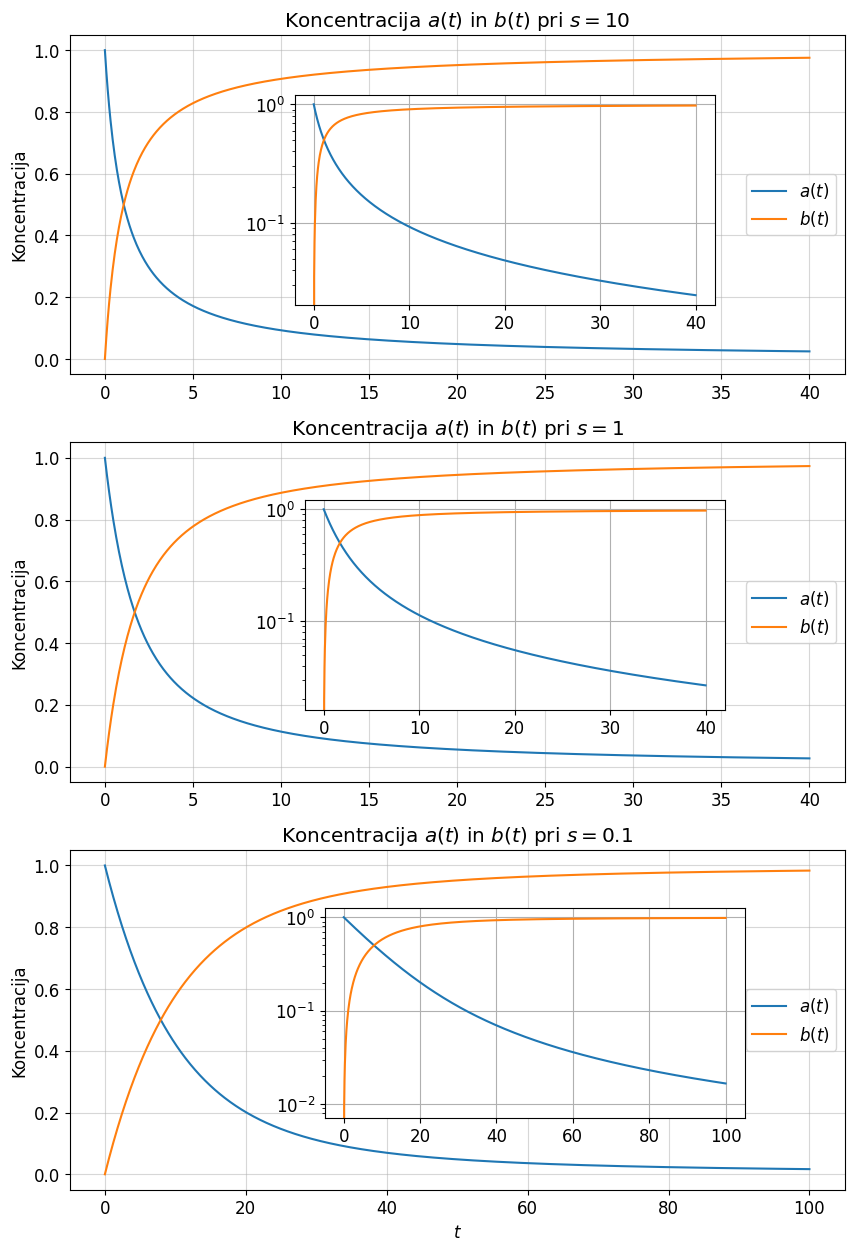
\includegraphics[width=15cm]{binarna2.png}
\caption{Na sliki vidimo potek koncentracij $a$ in $b$ v odvisnosti od časa pri različnih vrednostih parametra $s$. Vrednosti so prikazane v linearni in logaritemski skali. Vidimo, da za manjše $s$ reakcija poteka več časa.}
\end{figure}

\newpage

\begin{figure}[h!]
\centering
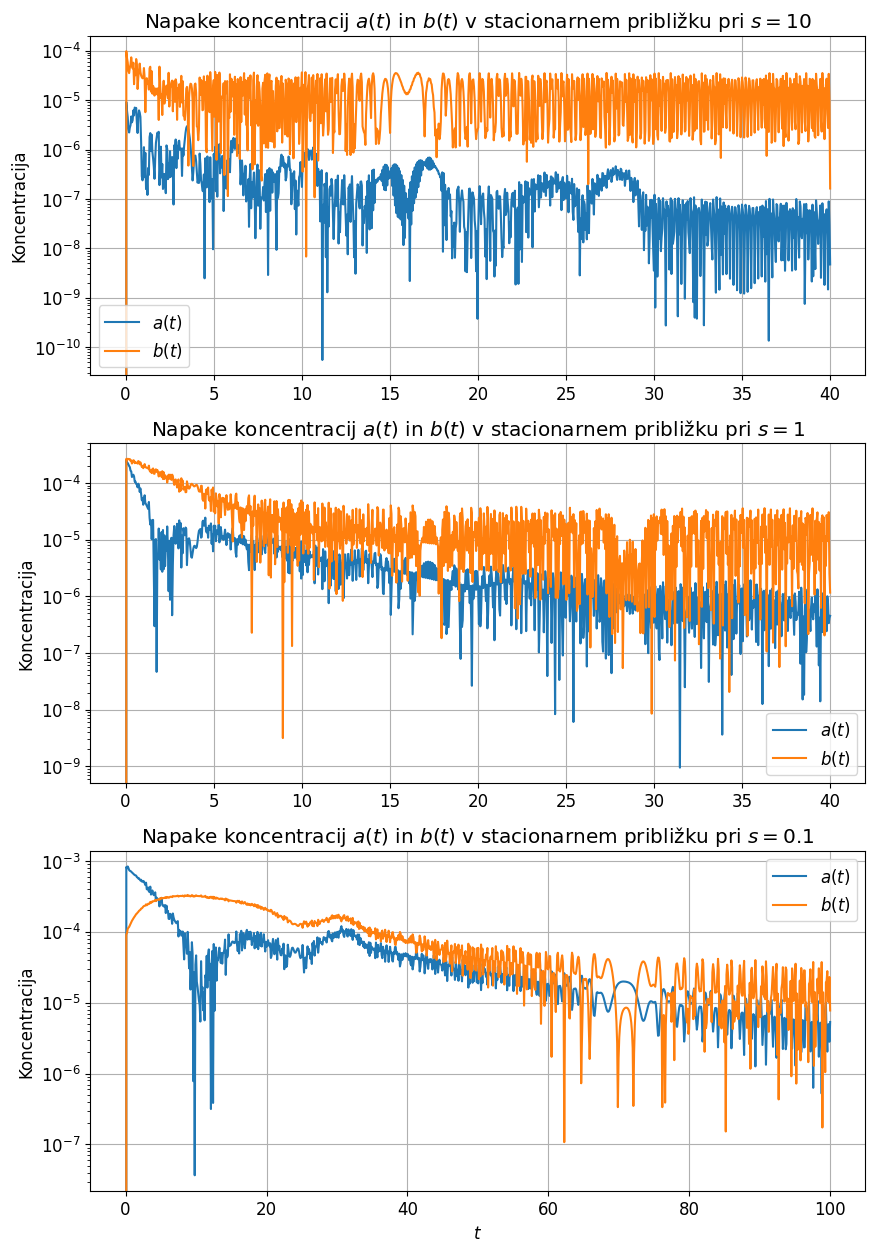
\includegraphics[width=15cm]{binarna3.png}
\caption{Na sliki vidimo napake koncentracij $a$ in $b$ pridobljenih z stacionarnim približkom v odvisnosti od časa. Za manjše vrednosti parametra $s$ so napake izračunanih koncentracij $a$ in $b$ večje, saj je tam stacionarni približek manj upravičen, kot v manjših vrednostih $s$. Upravičenost lahko razberemo iz slike 1.}
\end{figure}

\newpage

\section{Model reakcije z vodikovim bromidom}

Druga reakcija, ki si jo bomo ogledali je proces pridobivanja vodikovega bromida iz broma in vodika. Model reakcije $\ce{H2 + Br2 <=>[p][q] 2HBr}$ vključuje naslednje stopnje

\begin{align}
\ce{Br2 & <=>[p][q] Br + Br} \\
\ce{Br + H2 & <=>[r][s] HBr + H} \\
\ce{H + Br2 & ->[t] HBr + Br},
\end{align}
kjer so $p$, $q$, $r$, $s$ in $t$ parametri, ki določajo hitrost poteka določene reakcije. Zaradi lepše notacije pišimo koncentracije spojin in elementov kot

\[
u = [\ce{H2}], \quad v = [\ce{Br2}], \quad x = [\ce{HBr}], \quad y = [\ce{H}] \quad \text{in} \quad z = [\ce{Br}].
\]
Sedaj lahko zapišemo sistem diferencialnih enačb, ki ga določajo kemijske enačbe (12)-(14)

\begin{align}
\dot{u} &= sxy - ruz \\
\dot{v} &= qz^2 - pv - tvy \\
\dot{x} &= rzu - sxy + tyv \\
\dot{y} &= rzu - sxy - tyv \\
\dot{z} &= 2pv - 2qz^2 - ruz + sxy + tyv.
\end{align}

Vrednosti parametrov si izberemo $p=q=r=1$, $s=2$ in $t=5$. Na sliki 4 je prikazana rešitev sistema enačb (15)-(19) dobljena s funkcijo \texttt{solve\_ivp} in metodo \texttt{DOP853} za različne začetne pogoje $u/v$. Poteki reakcij se zelo razlikujejo. Vidimo, da največ končnega produkta $x$ nastane pri začetnem pogoju $u/v=1$. Pri drugih začetnih pogojih je končnega produkta po reakciji zelo malo.

\subsection{Stacionarni približek}

Podobno kot v prejšnjem poglavju poskusimo s stacionarnim približkom priti do kakšnega lepšega rezultata. Odvoda vmesnih produktov postavimo na 0 $\dot{y} = \dot{z} = 0$ in iz teh dveh enačb nato izpostavimo $y$ in $z$ in ju vstavimo v druge tri enačbe. Po nekaj računanja dobimo sistem diferencialnih enačb

\begin{align}
\dot{x} &= k \frac{u\sqrt{v}}{m+\frac{x}{v}} \\
\dot{u} &= -\frac{k}{2} \frac{u\sqrt{v}}{m+\frac{x}{v}} \\
\dot{v} &= -\frac{k}{2} \frac{u\sqrt{v}}{m+\frac{x}{v}},
\end{align}
kjer je $k = \frac{2tr}{s}\sqrt{\frac{p}{q}} = 5$ in $m=\frac{t}{s} = 2.5$. Na sliki 5 je prikazana dobljena rešitev sistema enačb (20)-(22). Na prvi videz sta pri začetnem pogoju $u/v=1$ poteka reakcij podobna. Vendar slika 6 prikazuje odstopanja rešitve približka stacionarnega stanja od eksaktne rešitve. Vidimo, da napake koncentracije končnega produkta $x$ segajo vse do $20\%$. V prvem poglavju je stacionarni približek bil bolj upravičen kot tukaj. Očitno vidimo, da je končna koncentracija produkta $x$ odvisna od začetnega razmerja $u/v$. Graf, ki prikazuje to odvisnost je prikazan na sliki 7. Gledal sem maksimum koncentracije $x$ izračunan za eksaktno rešitev in za približek stcionarnega stanja v časih od 0 do 1000.

\newpage

\begin{figure}[h!]
\centering
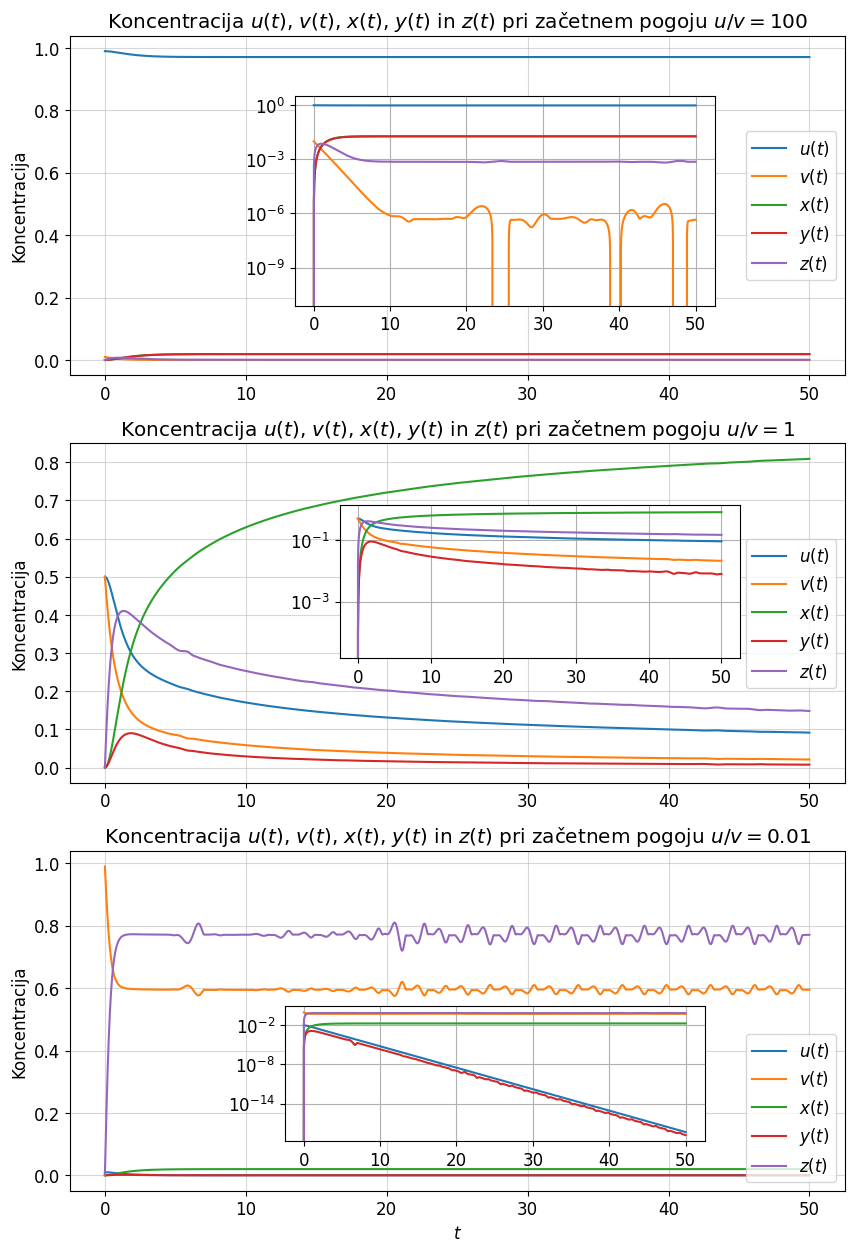
\includegraphics[width=15cm]{bromid1.png}
\caption{Na sliki vidimo potek koncentracij $u$, $v$, $x$, $y$ in $z$ v odvisnosti od časa pri različnem začetnem pogoju $u/v$. Vrednosti so prikazane v linearni in logaritemski skali. Vidimo, da največ končnega produkta $x$ nastane pri začetnem pogoju $u/v = 1$.}
\end{figure}

\newpage

\begin{figure}[h!]
\centering
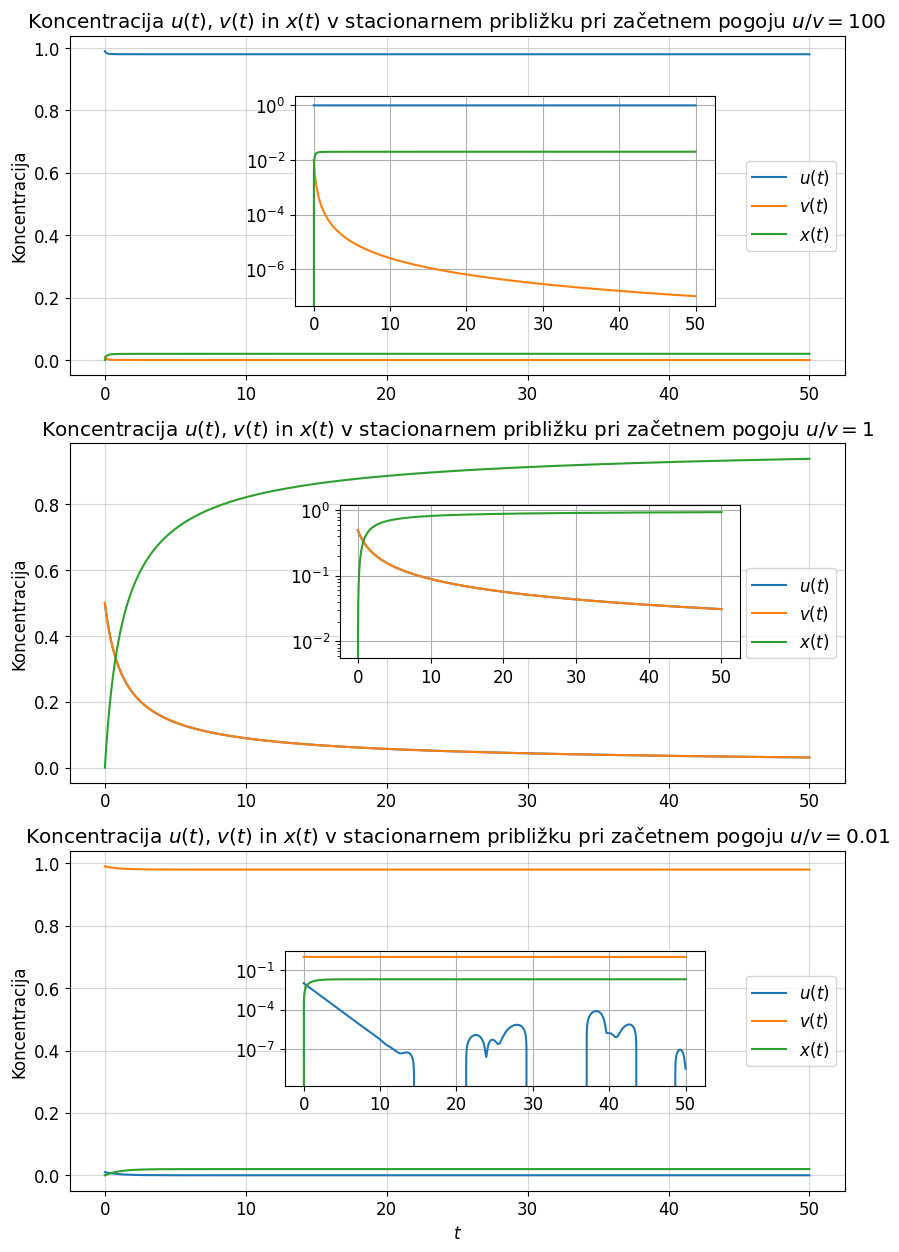
\includegraphics[width=15cm]{bromid2.png}
\caption{Na sliki vidimo potek koncentracij $u$, $v$ in $x$ v odvisnosti od časa pri različnem začetnem pogoju $u/v$ izračunenih v stacionarnem približku. Vrednosti so prikazane v linearni in logaritemski skali. Vidimo, da največ končnega produkta $x$ nastane pri začetnem pogoju $u/v = 1$.}
\end{figure}

\newpage

\begin{figure}[h!]
\centering
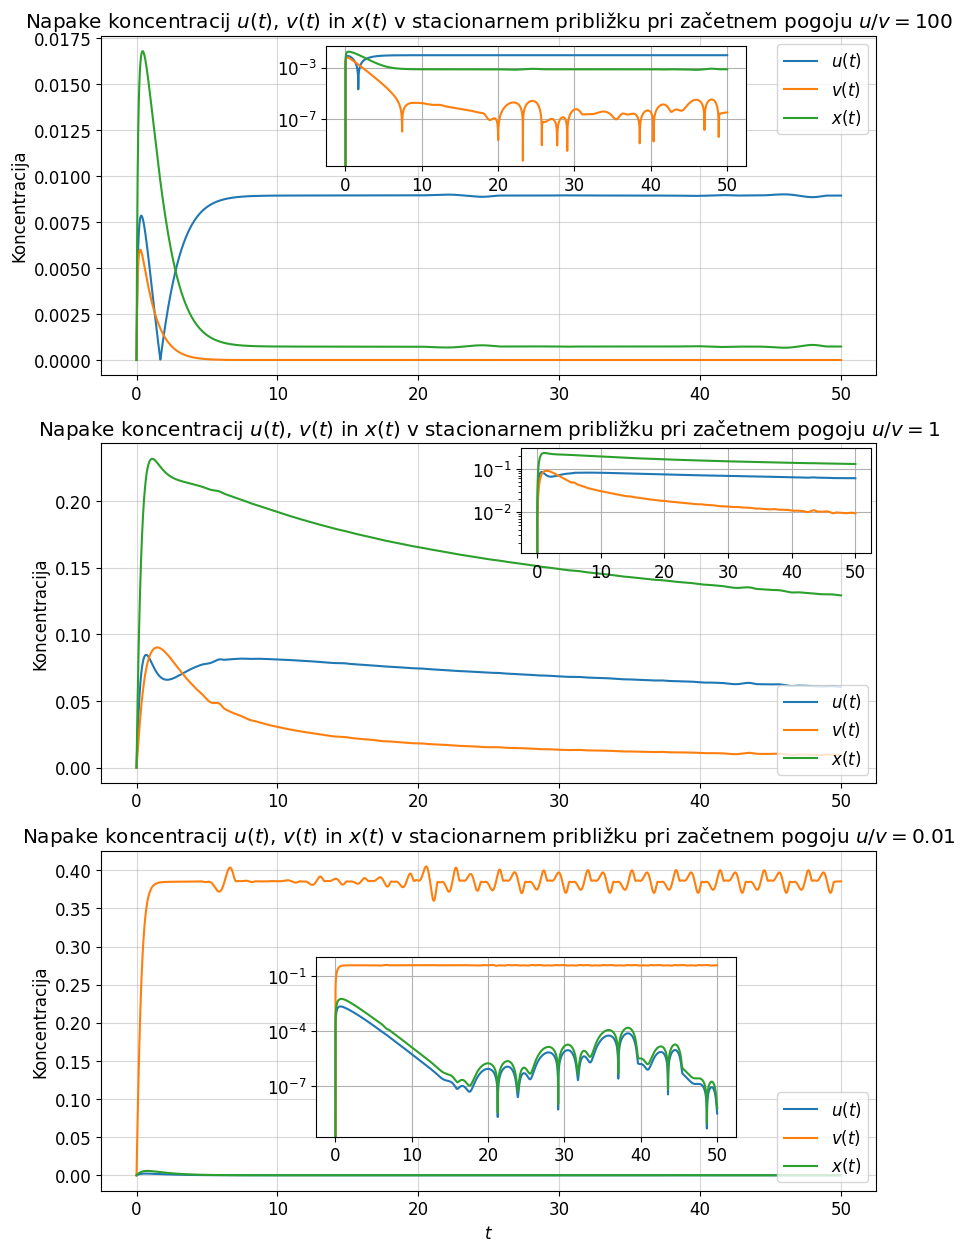
\includegraphics[width=15cm]{bromid3.png}
\caption{Na sliki vidimo napake koncentracij $u$, $v$ in $x$ pridobljenih s stacionarnim približkom v odvisnosti od časa pri različnem začetnem pogoju $u/v$. Vrednosti so prikazane v linearni in logaritemski skali.}
\end{figure}

\newpage

\begin{figure}[h!]
\centering
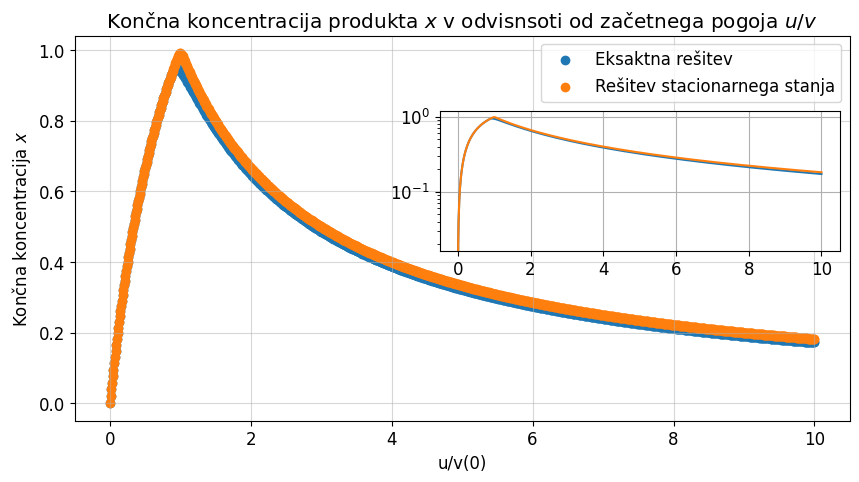
\includegraphics[width=15cm]{bromid4.png}
\caption{Končna koncentracija produkta $x$ v odvisnosti od začetnega pogoja $u/v$ za eksaktno rešitev in rešitev s približkom stacionarnega stanja.}
\end{figure}

\subsection{Primešavanje končnega produkta}

Na sliki 8 je prikazan časovni potek koncentracije končnega produkta $x$ v odvisnosti od časa za več različnih začetnih vrednosti $x(0)$ med $0\%$ začetne snovi, do $50\%$ začetne snovi. Vidimo, da čas v katerem poteče reakcija do konca ni pretežno odvisen od začetne vrednosti končnega produkta. Na sliki je koncentracija $x(t)$ izračunana po eksaktni poti, saj je ta pri mojih izbranih parametrih precej natančnejša.

\begin{figure}[h!]
\centering
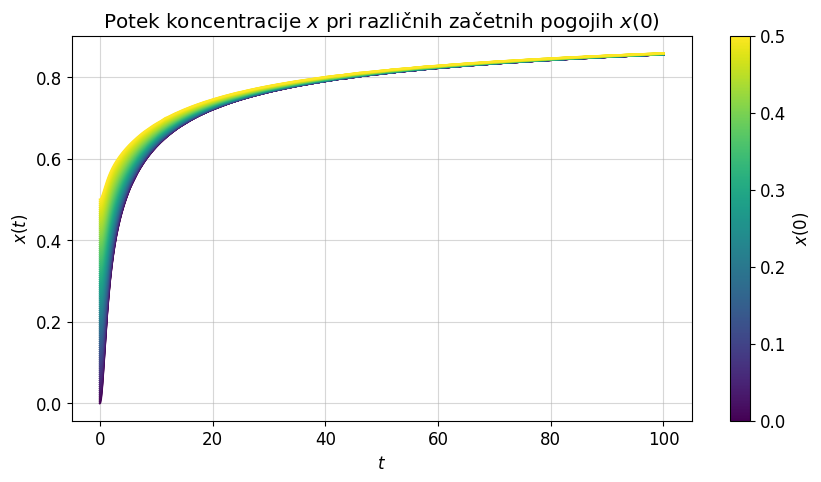
\includegraphics[width=15cm]{bromid5.png}
\caption{Koncentracija produkta $x$ v odvisnosti od časa pri $u/v=1$ za eksaktno rešitev pri več različnih začetnih pogojih $x(0)$.}
\end{figure}

\newpage

\subsection{Merjenje konstant k in m}

Konstanti $k$ in $m$ najlažje izmerimo tako, da najprej gledamo začetni koeficient, če nimamo na začetku nič $x$. Enačba (20) se torej poenostavi v

\begin{equation}
\dot{x} = \frac{k}{m} u \sqrt{v}.
\end{equation}
Če poznamo začetne vrednosti $\dot{x}$, $v$, in $u$ lahko določimo razlerje $\frac{k}{m}$. Nato poskus ponovio z veliko začetno koncentracijo $x$ in se enačba (20) poenostavi v

\begin{equation}
\dot{x} = \frac{kuv^{3/2}}{x}.
\end{equation}
Če poznamo začetne vrednosti $\dot{x}$, $v$, in $u$ lahko določimo $k$. S pomočjo razmerja $\frac{k}{m}$ pa nato določimo še $m$.


\section{Kemijske ure}

Kemijske ure so reakcije, ki stečejo s predvidljivim in ponavadi ostrim časovnim zamikom. Primer takšne reakcije je jodova ura, ki v eni izmed izvedb temelji na ravnotežju naslednjih reakcij:

\begin{align}
\ce{S2O8^{2-} + 2I- ->[r] I2 + 2SO4^{2-}} \\
\ce{2S2O3^{2-} + I2 ->[p] 2I- + S4O6^{2-}}.
\end{align}
Druga reakcija je bistveno hitrejša od prve, mehanizem merjenja časa pa je enakomerno porabljanje tiosulfata $\ce{2S2O3^{2-}}$. Če je persulfat $\ce{2S2O8^{2-}}$ v prebitku, lahko za aktivne spremenljivke vzamemo le $[\ce{I-}]$, $[\ce{I2}]$ in $[\ce{2S2O3^{2-}}]$. Takrat lahko pišemo

\begin{align}
\dot{[\ce{I-}]} &= -r [\ce{I-}]^2 + p[\ce{I2}][\ce{2S2O3^{2-}}]^2 \\
\dot{[\ce{I2}]} &= r [\ce{I-}]^2 - p[\ce{I2}][\ce{2S2O3^{2-}}]^2 \\
\dot{[\ce{2S2O3^{2-}}]} &= -p[\ce{I2}][\ce{2S2O3^{2-}}]^2.
\end{align}

Enačbo delimo z $r$ in uvedemo nove spremenljivke
\[
x = [\ce{I-}], \quad y = [\ce{I2}], \quad z =[\ce{2S2O3^{2-}}], \quad k = \frac{p}{r}
\quad \text{in} \quad t = t'r
\]
ter problem prepišemo

\begin{align}
\dot{x} = -x^2 + kyz^2 \\
\dot{y} = x^2 - kyz^2 \\
\dot{z} = yz^2,
\end{align}
kjer je s piko $\dot{}$ označen odvod po času $t$. Na sliki 9 so kompaktno prikazani rezultati rešitve sistema enačb (30)-(32). Na sliki lahko vidimo časovne poteke koncentracij $x$, $y$ in $z$. Na grafih vidimo, da so za večje vrednosti $k$ prehodi bolj ostri in hitrejši. To si želimo, saj imamo na ta način manj prosora za napako pri štopanju z štoparico in očesom.

\newpage

\begin{figure}[h!]
\centering
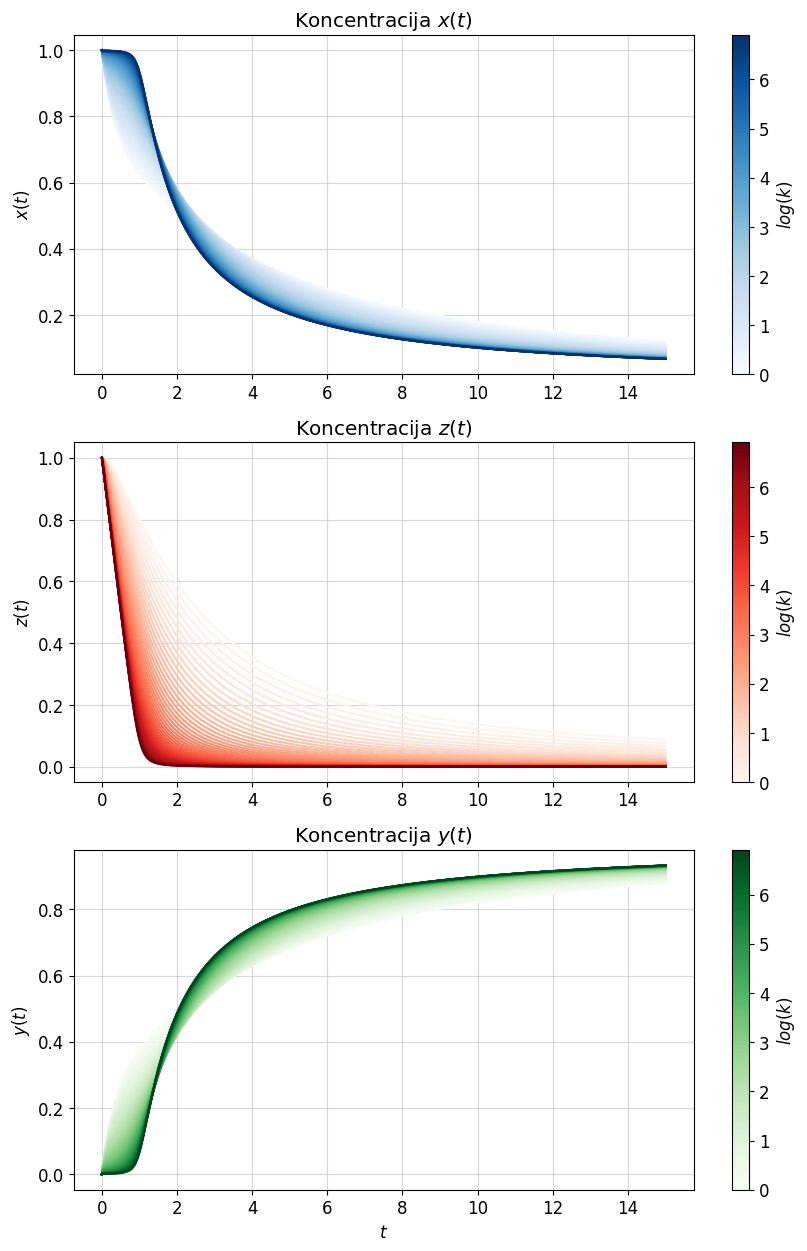
\includegraphics[width=14cm]{ura1.png}
\caption{Koncentracija $x$, $y$ in $z$ v odvisnosti od časa pri različnih vrednostih parametra $k$. Na grafih vidimo, da so za večje vrednosti $k$ prehodi bolj ostri in hitrejši.}
\end{figure}

\newpage

Na sliki 10 je na zgornjem grafu prikazan čas $\tau$ v katerem koncentracija $y(t)$ doseže polovico svoje končne vrednosti v odvisnosti od parametra $k$. Če poznamo razmerje hitrosti reakcij $k$ lahko sedaj iz grafa $\tau(k)$ razberemo čas $\tau$. Ta čas $\tau$ nato delimo s hitrostjo prve reakcije $r$ in dobimo dejanski čas $t'$ v enotah s za katerekoli hitrosti reakcij $r$ in $p$. Na spodnjem grafu pa je prikazan čas $\Delta \tau$. To je čas, ki ga $y(t)$ potrebuje, da pride iz $20\%$ do $80\%$ svoje končne vrednosti. Če s štoparico in očesom merimo čas, bi večji $\Delta\tau$ pomenil več prostora za napako.

\begin{figure}[h!]
\centering
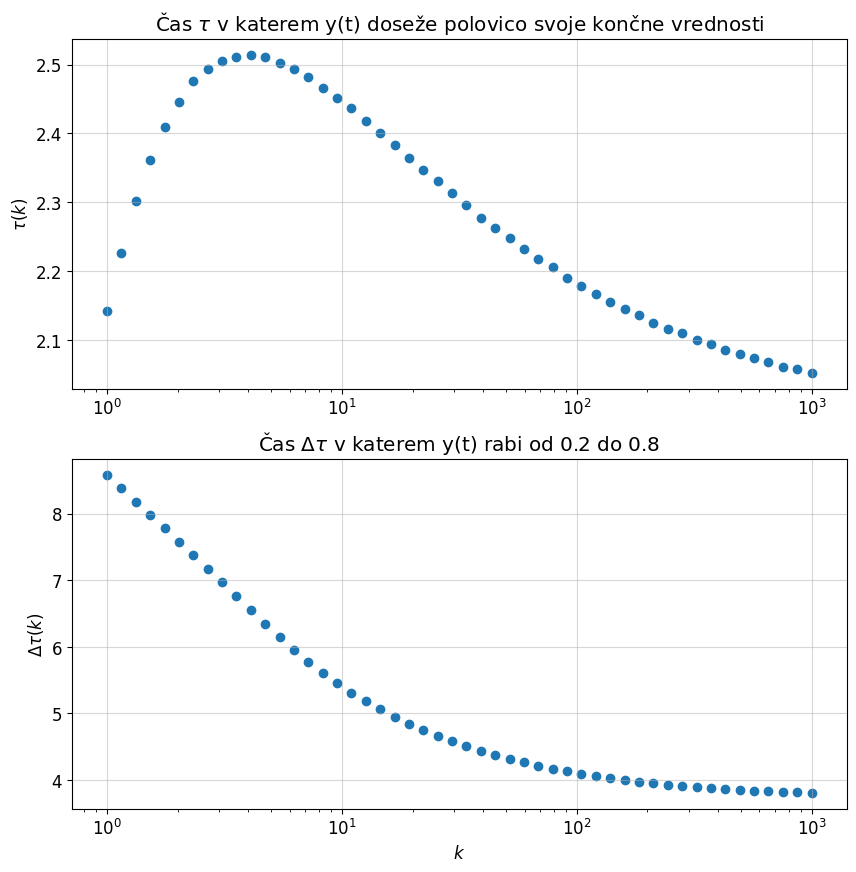
\includegraphics[width=14cm]{ura2.png}
\caption{Grafa prikazujeta čas $\tau$ v katerem $y(t)$ doseže polovico svoje končne vrednosti in čas $\Delta\tau$. To je čas, ki ga $y(t)$ potrebuje, da pride iz $20\%$ do $80\%$ svoje končne vrednosti.}
\end{figure}

\section{Zaključek}

Naučili smo se modelirati potek koncentracij spojin oz. elementov iz kemijskih enačb. Spoznali smo aproksimacijo stacionarnega stanja in njeno uporabnost.

\end{document}